% ========================================== %
% White Paper on the Wownero Cryptocurrency
% Written For Class Assignment
% ========================================== %

\documentclass[a4paper,11pt,oneside,onecolumn]{article}
\usepackage[portrait, margin=3cm]{geometry}

% Modify page color
% ========================================== %
\usepackage[svgnames]{xcolor}
\definecolor{doc_purple}{HTML}{590059}
\definecolor{doc_piss}{HTML}{FFFFB2}
\pagecolor{doc_piss}
\color{doc_purple}
% ========================================== %


% Modify Footnotes
% ========================================== %
% Anchor footnotes to bottom of page
\usepackage[bottom]{footmisc}
% Use dagger symbol for footnotes
\renewcommand*{\thefootnote}{\textdagger\arabic{footnote}}
% Make footnote index reset per page
\usepackage{perpage}
\MakePerPage{footnote}
% Adjust footnote rule line
\renewcommand{\footnoterule}{
  \kern -3pt
  \hrule width 5cm height 0.5pt
  \kern 2pt
}
% ========================================== %

% Bibliography Setup
% ========================================== %
\newcommand{\citecountenabled}{false}
\usepackage[
    backend=biber,
    style=numeric,
    sorting=none,
    citecounter=\citecountenabled,
    backref=\citecountenabled
]{biblatex} 
\addbibresource{sources.bib}
% Make citation markers smaller
\let\oldcite\cite
\renewcommand*\cite[1]{{\scriptsize\oldcite{#1}}}
% Make Bibliography font smaller
\renewcommand*{\bibfont}{\small}
\iffalse
\renewbibmacro*{pageref}{\\\textsubscript{
    \printtext{Cited \arabic{citecounter} time\ifnumgreater{\value{citecounter}}{1}{s}{}}%
    \setunit{\addspace} on page\ifnumgreater{\value{pageref}}{1}{s}{}%
    \printlist[pageref][-\value{listtotal}]{pageref}}
}
\fi
% ========================================== %

% In text links (such as citations and footnotes)
\usepackage{hyperref}


% Figures and captions
% ========================================== %
\usepackage{graphicx}
\graphicspath{{./figs}}
\usepackage[justification=centering]{caption}
% Allow blocking float on figures
\usepackage{float}
% ========================================== %


% Drawing and image positioning
% ========================================== %
\usepackage{tikz}
% ========================================== %


% Mathematical Symbols & Forumlas
% ========================================== %
\usepackage{amsmath}
\usepackage{amssymb}
\usepackage{amsfonts}
\usepackage{bm}
% ========================================== %


% Modify Itemize and Enumerate
\usepackage{enumitem}
% ========================================== %
% Reduce List spacing
\setlist{noitemsep}
% or \setlist{\nosep} to remove space around list too
% ========================================== %


% Prevent \url's from extending past margin
\usepackage{xurl}


% Redact sensitive text
% ========================================== %
% Switch the comments to toggle censor
% \usepackage{censor}
\newcommand\censor{}
% ========================================== %


% For lettered sections
%\renewcommand{\thesubsection}{\Alph{subsection}}


% Setup Title
% ========================================== %
\newcommand{\doctitle}{WOWNote v 6.9}
\title{\doctitle}

\newcommand{\authorname}{\censor{RootInit}}
\newcommand{\authoremail}{\censor{init.cx}}
\author{\authorname\\\authoremail}
%\author{\censor\authorname \\ \censor\authoremail}
%\newcommand{\authoremail}{email@email.com}

\newcommand{\docdate}{\today}
\date{\censor\docdate}
% ========================================== %

\begin{document}

% Header on each page
% ========================================== %
%\pagestyle{fancy}
%\setlength{\headheight}{15pt}
%\fancyhead[L]{003128756}
%\fancyhead[C]{\authorname}
%\fancyhead[R]{\docdate}
% ========================================== %

% Print table of contents
% ========================================== %
%\tableofcontents
% ========================================== %

% Print title block
% ========================================== %
\maketitle
% ========================================== %

% Document Sections
% ========================================== %
\section{Introduction}
``Monero''\cite{monero_about,zero2monero,monero_repo} has been a successful derivative of the CryptoNote\cite{CryptoNote} proof-of-concept cryptocurrency and has become the most popular privacy focused p2p digital currency. Both digital privacy advocates and the general cryptocurrency using public have come to appreciate its private and anonymous transactions and ASIC resistant proof-of-work algorithm. Today, the Monero user base is growing at a steady pace\cite{acceptedhere}; users are attracted to the low transaction fees and enhanced anonymity provided by its ``transaction mixing'' and ``stealth addresses''\cite{monerohow_btc_vs} and merchants value its predicted emission and fast transaction speed\footnote{\textbf{Transaction speed} is conditional on the number of confirmations and the network congestion level.} due to the two-minute block time. Monero has effectively proven that electronic cash transactions can be as, or more, private as paper money with a much higher degree of fungibility\footnote{\textbf{Fungibility} is the attribute of being indistinguishable from one another\cite{moneropedia}. For instance transparent blockchains result in ``tainted'' or ``dirty'' currency as coins are distinctly identifiable.} and with easily verifiable proof of payment\cite{proofofpayment}.

Unfortunately, Monero suffers from overwhelming practicality and over-seriousness. ``Wownero,''\cite{wowbsite} a digital currency forked from Monero\cite{monero_repo, wowrepo} seeks to solve this problem. Wownero is a memecoin primarily targeted toward transactions such as betting on snail races and tipping meme creators, but also a fully functional digital currency capable of being used in any financial transaction\cite{wowbsite}. Because of Wownero's less critical\textsubscript{[citation needed]} nature the community enjoys less stringent testing and validation requirements resulting in faster release of new features, lower block confirmation requirements, and much more playful presentation and branding\cite{slimecash}.

This document is intended to serve as an addendum to the existing Wownero white paper (\url{wownero.org/whitepaper.pdf}) and attempts to provide a brief synopsis of the core technologies Wownero (and Monero) utilize. A brief history of Wownero and a brief synopsis of core technologies will be provided. The Wownero blockchain, Proof-of-Work algorithm, and privacy enhancing features will be summarized in respective sections. 

While I have made a strong effort to provide accurate information, my lack of expertise in cryptography and the level of abstraction required to sufficiently condense the material may result in inaccuracies.

\begin{figure}[H]
    \centering
    
\includegraphics[height=60px]{logos}
    \caption{
        Monero (left) and Wownero (right) Logos
    }
    \label{fig:logos}
\end{figure}



\section{Wownero History}
Wonero is a Monero software fork created by John Winter Murphy (``jwinterm'')\cite{wowdere_dev} in response to, and with the goal of beating, ``MoneroV''\cite{jwinterview}. Wownero started as a casual discussion between John Murphy and his friend, Carty Sewill, about a hypothetical meme coin with some of the same features as MoneroV but as a fully legitimate and functional non-scam coin\cite{jwinterview}.

MoneroV, announced February 2018, was another fork of Monero with the main defining feature of having finite supply and no tail emission\cite{monerov}. In addition to the software, MoneroV also forked the Monero blockchain giving all existing Monero users 10 ``XMV'' for each ``XMR''\footnote{\textbf{XMR} is the common shorthand used for Monero similar to Wownero's abbreviation of ``WOW''.} they held.
Because MoneroV presold coins to investors, claimed a large percentage of coins as a ``dev tax,'' it is widely believed to have been entirely a scam\cite{monerov_scam,monerov}. 


Wownero was successfully launched on April 1st 2018 achieving their goal of launching ahead of MoneroV\cite{jwinterview}. Carty Sewill designed the original logo (Figure \ref{fig:logos}) and artwork used for the project\cite{jwinterview}. Like MoneroV, Wownero featured a limited max supply of approximately 10x the amount of Monero coins, but without any scammy pre-mined coins or ICO\footnote{\textbf{ICO} or Initial Coin Offering refers to a presale of a token offered to investors before launch} and utilized its own unique Genesis block\footnote{A \textbf{genesis block} is the initial block in the blockchain.} making it an entirely separate cryptocurrency from Monero.

Wownero was described by jwinterm in a personal communication as ``to Monero what Dogecoin is to Bitcoin'' (2023 \cite{jwinterview}). True to this claim, Wownero, has predominantly been used by a largely meme based community and, like Dogecoin, Wownero is categorized by many as a ``shitcoin'' though some may (sarcastically) disagree as shown in \texttt{Figure \ref{fig:theshitmeme}}.

\begin{figure}[h]
    \centering
    
\includegraphics[width=300px]{theshit}
    \caption{
        A meme facetiously disputing Wownero's status as a ``shitcoin.''\\
        Image source \texttt{suchwow.xyz} credit \emph{``trichom''}
    }
    \label{fig:theshitmeme}
\end{figure}

A strong and active community has formed around Wownero and developed a full software ecosystem to make Wownero a more functional and user-friendly coin. Community projects include:

\begin{itemize}
    \item GUI, TUI, and VR wallets\cite{wowlet}.
    \item Blockchain explorers\cite{muchwowblocks}.
    \item Informational websites\cite{wowbsite,slimecash}.
    \item Promotional memes, artwork, and stickers\cite{suchwow}.
    \item A Discord server, subreddit, and dedicated forum\cite{wowrum}.
    \item A privately hosted Git server for software development collaboration\cite{wowrepo}.
\end{itemize}

Monero and Wownero have always had trouble getting listed on most major exchanges as such exchanges generally avoid privacy coins both for fear of future regulatory legislation, and because centralized exchanges (which require ID verification) are not likely to be popular with the privacy coin demographic. Wownero has been primarily traded through ``TradeOgre'' and has reciently been listed on various exchanges including ``MajesticBank,'' ``LocalMonero,'' and ``Agoradesk'' \cite{jwinterview}. The Wownero community is optimistic regarding near future listings on other exchanges.


\section{Blockchain}
A blockchain is a decentralized and distributed digital ledger that records all transactions\cite{moneropedia}. This core technology that makes cryptocurrency possible was originally proposed in 2008 for ``Bitcoin'' by a person or group under pseudonym ``Satoshi Nakamoto''\cite{bitcoin_whitepaper}. The blockchain is stored on a network of nodes (computers running the blockchain's daemon\footnote{A \textbf{Daemon} is a program which runs as a background service and communicates with other nodes.} software) with new transactions and blocks being propagated via a peer-to-peer (P2P) protocol\cite{ledger_transactions}. An LMDB (Lightning Memory-Mapped Database) is used for both Monero and Wownero blockchain data storage\cite{monero_repo,wowrepo}.

% ------------------------------------------ %
\subsection{Transaction Process}
When a transaction is initiated it is broadcast to the network and stored in each node's transaction cache, also known as a ``memory pool,'' if the transaction passes validation checks\cite{ledger_transactions}. These transaction validation checks typically check factors such as confirming the money exists, it has only been sent once, it is being sent by the address which owns it, the transaction received amount equals the input, and the transaction is correctly formatted\cite{zero2monero}.
``Miner'' nodes attempt to create a new ``block'' from this transaction queue and when successful a new block is added to the blockchain\cite{ledger_transactions} containing a list of hashed\footnote{\textbf{``Hashing''} refers to the use of a mathematical algorithm to produce a numeric value that is representative of input data\cite{glossary}.} transactions.

Most blockchains enforce a multiple confirmation requirement before received funds can be used in a transaction again (``unlock time'')\cite{wikipedia_crypto}. This prevents double-spend and similar attacks by making the transaction more difficult to reverse as an attacker would need to overwrite multiple blocks on the blockchain. This becomes exponentially more difficult to do as more confirmations are added. Monero requires 10 confirmations\cite{monero_transactiontime} before funds are unlocked while Wownero requires only 4 confirmations\cite{wowrepo}. For CryptoNight protocol blockchains, like Monero and Wownero, it also serves to prevent people from making multiple transactions at the same block height which may compromise ring signature based transaction obfuscation.

It should be noted that for small transactions it may not be necessary to wait for the full blockchain confirmations and in some cases just the validated initial broadcast may be sufficient to approve a sale.

% ------------------------------------------ %
\subsection{Blocks}
Blocks are created by miner nodes and the ``block time'' (average time interval between block creation) is controlled by adjusting the proof-of-work algorithm difficulty against the hashrate\footnote{\textbf{Hashrate} is a measure of the computational power of a cryptocurrency network.} of the network\cite{randomx_repo,wikipedia_crypto}. The \emph{average} block time for Monero is pre-set at 2 minutes\cite{monero_about} as opposed to 5 minutes for Wownero\cite{wowrepo}.

In addition to a list of hashed transactions, each block will contain header information and a new hashed ``coinbase transaction'' which rewards the miner for creating the block\cite{monero_blocks, ledger_transactions}. The block header data will include a hash of the previous block ensuring that the blockchain must remain a sequential and complete ``chain''\cite{zero2monero,wikipedia_crypto}. This ensures that previous block alteration or removal is impossible without replacement of all subsequent blocks\cite{zero2monero}.

Because it is possible for more transactions to occur between blocks than would fit within the block size limit,\footnote{\textbf{Block size limit} is a pre-set but not hard-coded parameter\cite{CryptoNote}. Note: Both Monero and Wownero have an adaptive block size limit calculated dynamically\cite{monero_transactiontime}.} transactions may remain in the queue until a later block. To prevent transaction spam, Monero has a dynamically calculated minimum fee on all transactions, however, if a sender needs to ensure their transaction is added to the earliest possible block they can raise the fee above the minimum\cite{zero2monero}. Because the transaction fee is given to the miner who creates the block, transactions offering a higher fee take priority in the queue.
To prevent miners from producing unnecessarily large blocks (such as by padding to max size with zero value transactions) an excessive block size penalty is subtracted from the block reward\cite{CryptoNote}. This balances with the transaction fee reward to create a stable equilibrium of average block sizes.

% ------------------------------------------ %
\subsection{Outputs}
Units of a cryptocurrency can be split into very small fractional amounts though there is a finite limit called ``atomic units.'' For Monero the atomic unit size is \texttt{0.000000000001} XMR or one ``piconero''\cite{moneropedia}.

Because it would be impractical to track the movement of each of these atomic units individually, an ``output'' and ``input'' based system is used instead\cite{bitcoin_whitepaper}. These outputs combine amounts of currency into single units, similar to how a \$10 bill combines the value of 1000 pennies\cite{monero_outputs}. If no single output is large enough to cover a transaction they can be combined, however there are always at most two outputs per transaction comprising the payment amount and the ``change'' returned to the sender\cite{bitcoin_whitepaper}. The one drawback to this system is that, as outputs are ``locked'' while a transaction is taking place and pending sufficient confirmations, a user lacking multiple outputs will be unable to send another transaction until the first one is fully confirmed. This is a rare issue however as almost all frequent users will have multiple outputs and the input output system is managed invisibly to the end user by the wallet software\cite{monero_outputs}.

% ------------------------------------------ %
\subsection{Emission}
Both Monero and Wownero had no premine, instamine, or presale of any kind to ensure a fair and even distribution\cite{monero_about, wowbsite}. Monero had irregular emission with block rewards steadily decreasing until they reached a flat 0.6 XMR block reward which will continue in perpetuity\cite{monero_faq}. Wownero took a different approach with a total supply of 184,467,440 coins to be mined over ~50 years and no tail emission\cite{wowrepo}. This may be an issue long term as without an incentive to mine the security of the network could be reduced\cite{zero2monero}.

% ------------------------------------------ %
\subsection{Blockchain Upgrades}
Both Monero and Wownero utilize a ``hard fork'' mechanism to implement scheduled software upgrades into their networks\cite{wowrepo,monero_repo}. A hard fork occurs when a majority of nodes no longer accept older versions of the blockchain\cite{hard_fork}. In the case of Monero and Wownero this has only occurred due to official changes to implement new features such as new proof-of-work algorithms or implementation of ``bulletproofs''\cite{monero_repo}.

In a hard fork the blockchain becomes split into an old and new version of the blockchain\cite{hard_fork}. Because of this it is possible for an official hard fork to be rejected by nodes which do not accept the changes which leads to a split. This has happened with other cryptocurrencies such as ``Etherium Classic'' which was formed in 2016 due to differences of opinion on whether a smart contract hack should be rolled back\cite{eth_classic}. Monero and Wownero have prevented this from occurring (so far) through clear communication, ensuring there is broad favorable consensus regarding an upgrade before an update is released\cite{monero_upgrades}. Because only changes accepted almost unanimously are implemented a ``non-contentious hard-fork'' occurs in which the old blockchain dies off due to a lack of nodes running the older version.

Some changes, referred to as ``soft forks'', can occur while remaining backwards compatible with the original blockchain. These changes require only miner nodes to update, and normal nodes remain unaffected\cite{soft_fork}. 

To the end user all upgrades require only a simple software update of the client software\cite{monero_upgrades}.

% ------------------------------------------ %
\subsection{Consensus}
Because of the decentralized, peer-to-peer, node based nature of cryptocurrency, maintaining consensus between the distributed nodes of the network is of critical importance. A majority of nodes must agree on the same blockchain, block creation structure, and transaction rules in order to prevent malicious actors from exploiting the network. This is achieved through the use of consensus algorithms, which enable the nodes of the network to agree on a shared version of the blockchain.

To ensure every node uses the same blockchain, the chain with the highest cumulative difficulty\footnote{\textbf{Cumulative difficulty} refers to the total difficulty required to mine every block in the chain.} is considered to be the legitimate version\cite{zero2monero}. This ensures that, in order to force an alteration to the transaction history, an attacker must create a fork of the blockchain with higher total difficulty than the original. This would in almost all cases require the attacker to control over 50\% of the total network mining hashrate to grow faster than the main chain\cite{zero2monero}.

Both Monero and Wownero utilize a proof-of-work algorithm (described in a later section) to maintain block consensus\cite{monero_about,wowbsite}. Other cryptocurrencies may use proof-of-stake (in which block validators are chosen based on their stake in the network\cite{concensus_algorithms}), proof-of-capacity (in which miners prove storage capacity instead of computational power), proof-of-authority (in which validators are chosen based on their reputation or identity), or any other algorithm.
\pagebreak


\section{Proof-of-Work}
``Proof-of-work,'' or PoW, is a type of consensus algorithm used in blockchain networks since Bitcoin\cite{wikipedia_crypto}. In this concensus algorithm transactions are validated and new blocks are added to the blockchain through a computational puzzle that must be solved by miners\cite{bitcoin_whitepaper}. While PoW has some drawbacks, such as high energy consumption, it remains one of the most widely-used and secure consensus algorithms in blockchain technology\cite{concensus_algorithms}.

\subsection{Early Proof-of-Work}
Not all proof-of-work algorithms are equal, however. The first proof-of-work algorithm used was a double SHA-256\footnote{\textbf{SHA-256} is a cryptographic hash function used for data integrity and authenticity verification in various computer security applications.} based function used in Bitcoin\cite{bitcoin_whitepaper}. This was intended to result in an egalitarian ``one-CPU-one-vote'' system\cite{bitcoin_whitepaper}.

Unfortunately, and likely unforeseen to Satoshi Nakamoto, the explosion of Bitcoin's popularity resulted in bitcoin mining ASICs\footnote{An \textbf{ASIC} or Application-Specific Integrated Circuit is a computer chip that is designed to perform a specific function with high speed and efficiency due to its specialized nature\cite{glossary}.} being developed and advances in GPU compute technology made GPUs much more efficient at mining blocks. Because of this CPU mining was rendered uncompetitive and mostly impractical giving a massive advantage, by orders of magnitude, to owners of ASIC mining rigs and GPU clusters\cite{randomx_article}.

\subsection{CryptoNight}
The CryptoNote protocol on proposed an algorithm, later dubbed ``CryptoNight'' which was intended to ``close the gap between CPU (majority) and GPU/FPGA/ASIC (minority) miners''\cite{CryptoNote}. This algorithm worked by utilizing a memory bound function which would be most efficient on CPUs due to the large L3 cache modern CPUs possess\cite{CryptoNote}. The 2 Mb of memory required by the CryptoNight algorithm was thought to be extremely difficult to develop an ASIC around and GPU processors do not have internal cache but rather rely on significantly slower memory on a separate chip\cite{CryptoNote}.

Ultimately CryptoNight failed in its efforts to provide ASIC resistance and ASICs capable of running the CryptoNight algorithm were developed\cite{CryptoNight}. Coins utilizing CryptoNight were forced to either accepted ASIC mining or switch to a different PoW algorithm.

Choosing the latter option, the Monero Research Lab upgraded the CryptoNight algorithm to v7, v8, and ``CryptoNight-R'' though all of these modifications were eventually defeated by improvements in ASIC technology\cite{CryptoNight}. The CryptoNight-R algorithm introduced a novel change of randomized integer math which was \emph{temporarily} very effective but only used in Monero between March 9, 2019 and November 30th 2019 as a new superior algorithm was internally developed specifically for use with Monero\cite{monero_repo}.

\subsection{RandomX}
Based on the same core principle of introducing randomness as CryptoNight-R, the Monero Research Lab developed an entirely new Proof-of-Work algorithm called ``RandomX'' with much stronger ASIC resistance while retaining the same private hashing as CryptoNight\cite{randomx_article}. Rather than rely on any single specific attribute of CPUs (such as cache size), RandomX instead is based on execution of random code inside a virtual machine\cite{randomx_repo}. RandomX has two modes with different memory requirements. A \emph{light} mode requiring only 256 MiB of memory (intended for normal nodes) to use for verification and a \emph{fast} mode requiring 2080 MiB of memory (intended for miner nodes)\cite{randomx_repo}. Because of the \emph{random} nature of the algorithm, only general purpose processors are capable of efficiently running it rendering ASICs theoretically impossible\cite{randomx_article}. Additionally, the high memory requirement for mining makes the mining software easily detectable by antivirus programs, low memory IoT devices unable to mine at all, and prevents web applications from mining covertly. These restrictions should reduce botnet\footnote{A \textbf{botnet} is a network of infected computers that are remotely controlled by a single attacker for malicious purposes.} mining, making it much harder for a malicious actor to obtain a high percentage of hashrate illegitimatly\cite{randomx_medium}.

Monero implemented the RandomX algorithm on November 30th 2019 as part of v12 update\cite{monero_repo}.

\subsection{Wownero}
Wownero likewise implemented a series of ASIC resistant POW algorithms including a slightly modified version of CryptoNight-R on the October 6th 2018 update codenamed ``Cool Cage''\cite{wowrepo}. They also briefly used a pseudorandom function ``CryptoNight/WOW'' from February 19th 2019 until the implementation of, RandomX based, ``RandomWOW'' which, due to lower testing requirements, they were able to implement ahead of Monero on the June 14th 2019 codename ``F For Fappening'' hard fork\cite{wowrepo}.

RandomWoW's differs from RandomX in that it uses a scratchpad (workspace memory)\cite{randomx_medium} size of only 1 MB compared to RandomX's 2 MB scratchpad size\cite{wowrepo}. RandomWOW also has a limit of 16 chained VM executions per hash to further increase program compilation difficulty for GPUs and ASICS\cite{wowrepo}.

Wownero took an additional step to promote decentralization through preventing public mining pools by requiring ``Miner Block Header Signing'' which requires miners to sign blocks with their private key\cite{wowrepo,jwinterview}. Because private keys cannot be shared without giving away full access to your wallet, this rendered Wownero solo and private pool mining only as of the July 4th 2021, ``Junkie Jeff,'' update\cite{wowrepo}.


\section{Privacy Enhancing Features}
Wownero is a privacy respecting memecoin\cite{wowbsite} and, as such, aims to provide users with strong anonymity and confidentiality. To achieve this, Wownero employs a range of privacy-enhancing features, including stealth addresses, ring signatures, RingCT, Dandelion+, and integration with TOR and I2P networks. The majority of these features were upstream inherited from Monero\cite{wowrepo,monero_repo}, but the Wownero developers have implemented some tweaks and modifications of their own.

% ------------------------------------------ %
\subsection{About Monero Addresses}
Conventional Bitcoin-like cryptocurrency addresses use a single key pair, similar to those used in \emph{RSA encryption}, but based on elliptic-curve cryptography\footnote{\textbf{Elliptic-curve cryptography} (ECC) uses the algebraic structure of elliptic curves over finite fields to perform cryptographic operations using smaller keys compared to conventional methods with the same level of security.}
\cite{zero2monero} rather than integer-factorization cryptography. Bitcoin wallet keys are generated using the ``Elliptic Curve Digital Signature Algorithm'' (ECDSA)\cite{ECDSA}. The key pair consists of a public key $(K)$ and a private key $(k)$ and, as is standard for asymmetric encryption, the public key is distributed freely (in the form of a derived address) while the private key must be carefully protected.

A standard Monero wallet address requires \emph{two} public-private key pairs. A view key $(K^v, k^v)$ and a spend key $(K^s, k^s)$\cite{monerodocs_addresses}. This double key pair system is a feature of CryptoNote coins and allows compartmentalization of access. For example, the view key can be shared to allow another party to audit incoming transactions and current balance without giving them the ability to send coins\cite{moneropedia}. Monero addresses are generated using the ``Edwards25519 Elliptic Curve'' signature scheme\cite{edwards_curve}.

I was curious what this curve looked like and plotted the positive and negative solutions to Curve25519 function in \texttt{Figure \ref{fig:curve}}. I do not believe this provides any greater understanding of the underlining mathematics, but now we know that it bears a striking visual similarity to a ``stick drawing'' of a fish.

\[y^2 = x^3+486662*x^2+x \implies \begin{cases}
y = +\sqrt{x^3 + 486662x^2 + x}\\
y = -\sqrt{x^3 + 486662x^2 + x}\end{cases}\]
\begin{figure}[H]
    \centering
    
\includegraphics[width=300px]{curve}
    \caption{
        The Edwards25519 Elliptic Curve\\
        Image credit: \emph{\authorname}
    }
    \label{fig:curve}
\end{figure}

In addition to the public spend and view keys, Monero and Wownero addresses also contains a ``network byte,'' which makes the address network type identifiable, and a checksum to make mistyped addresses easily detectable\cite{monerodocs_addresses}. The complete anatomy of a Monero address is as follows:\cite{monerodocs_addresses} 
\begin{enumerate}
    \item A 1 byte network byte located at index 0.
    \item A 32 byte public spend key located at index 1.
    \item A 32 byte public view key located at index 33.
    \item The first 4 bytes of a hash of the rest of the key located at index 65.
\end{enumerate}

Most cryptocurrencies use base58 encoding, originally developed for Bitcoin\cite{zero2monero}, for the final address. Base58 is similar to base64 but omits the characters \texttt{I, O, l, 0, +, and /} to avoid ambiguity when read\cite{monerodocs_addresses}. Monero addresses use a modified version of base58 which performs the encoding in 8 byte blocks and pads the final block with $1$s\cite{monerodocs_addresses}. This produces a fixed size output ensuring all addresses are of the same length.

\medskip\noindent
An example final Monero address after base58 encoding into a 95 character string:\\
{\scriptsize\texttt{84DwgAEGE3NBeocw33eoj8ZjomhVYTQEuUKew8yvYJMxgfdDU9Y91BBgtvAX6dJ3PddVJRwe3trRcNku3fMEHc3A7XYmDbC}}\\
A main chain standard Monero address will always have an \emph{4} or \emph{8} as the first character\footnote{It is entirely coincidental that the example Monero address starts with 84}.

\medskip\noindent
An example final 97 character Wownero address:\\
{\scriptsize\texttt{WW33MLqvVUJZxDs4WkqgHn4SkTdKFn6hb2VAN8MBvENjfu2iug6p3CSJPDsVpggtEDZd715Xj4zy2jabweCV6WmY2kF6NMuZE}}\\

It appears that the reason for the longer address is due to the use of two bytes to represent the network. Because of this, every standard main chain Wownero address will start with \emph{Wo} or \emph{WW} at the cost of a pre-encoding address size of 70 bytes in length \emph{not} 69.

% ------------------------------------------ %
\subsection{Stealth Addresses}
``Stealth addresses,'' also known as ``one-time addresses,''\cite{zero2monero} allow the recipient address written to the blockchain to be a unique single-use address that cannot be linked to the original address \cite{stack_stealth}. Without stealth addresses it would be possible for an observer monitoring blockchain transactions to link transactions through heuristic pattern analysis of received transactions. For instance, linking a purchase of Monero via credit card to all other received payments would be trivial and completely de-anonymize the user.

The procedure for generating a stealth address was first described in the CryptoNote white paper\cite{CryptoNote} and has become one of the core Monero and Wownero privacy enhancing technologies\cite{moneropedia}.

\subsubsection{Stealth Address Cryptography} \label{sec:SA_example}
An example usage of a stealth address in a transaction between a sender, ``Shinji'', and a recipient, ``Rei'', will be explained\cite{zero2monero,CryptoNote,}. 

\noindent\textbf{[Sender] Shinji's Steps}
\begin{enumerate}
    \item Shinji initiates a Wownero transaction sending an amount, $a$, addressed to an address Rei provided.
    \item The wallet software separates the address into Rei's public view and send keys $(K^v_R, K^s_R)$
    \item A random number $r$ is selected ($r \in _R\mathbb{Z}_l$)\footnote{The $R$ indicates random selection from the set}\footnote{$l$ indicates exclusion of the Curve25519 infinity points from the set}.
    \item A one time address $K^o$ is calculated as 
    \[K^o=\mathcal{H}_s(rK^v_R, a)G+K^s_R\]
    \footnote{$G$ refers to the Ed25519 ``generator point'' on the curve which is the first point after infinity.}\footnote{$\mathcal{H}_s$ refers to a one-way cryptographic hash function.}
    \item The transaction is sent to the network with the one-time address $K^o$ as the recipient along with the value of $rG$.
\end{enumerate}
\noindent\textbf{[Receiver] Rei's Steps}
\begin{enumerate}
    \item Rei's wallet checks every transaction using her private view key. $k^v_R$ and
    \begin{enumerate}
        \item Multiplies her private view key $k^v_R$ by $rG$ ($rK^v_R = k^v_RrG$)
        \item Derives the original public send key $K'^s_R$ with 
        \[K'^s_R = K^o-\mathcal{H}_s(rK^v_R,a)G\]
        \item Transactions in which the derived send key match Rei's public send key ($K'^s_R=K^s_R$) are addressed to Rei.
    \end{enumerate}
    \item Having identified the transaction, the public and private spend keys for the output can be calculated.
    \begin{align*}
        K^o &= \mathcal{H}_s(rK^v_R,a)G+K^s_R\\
        &= (\mathcal{H}_s(rK^v_R,a)+k^s_R)G\\
        k^o &=\mathcal{H}_s(rK^v_R,a)+k^s_R
    \end{align*}
    Rei can now spend the received amount as desired using the spend key pair $(K^o, k^o)$ and the amount is added to his balance by the wallet software.
\end{enumerate}

Stealth addresses can be used optionally with non CryptoNote based coins, including Bitcoin, if both parties wallets support the feature\cite{stack_stealth}. Monero and Wownero \emph{require} their use and their respective wallets perform this automatically and transparently\cite{moneropedia}.

\subsubsection{View Tags}
As of the Monero v15 update on August 13, 2022\cite{monero_repo} and Wownero's very recent April 1st update codenamed ``Kunty Karen''\cite{wowrepo}, a new noteworthy piece of data was added to blocks. ``View Tags'' are 1-byte ``tags'' added to each transaction using a shared secret generated by the sender using the address provided to them by the recipient\cite{monero_viewtag}. Because all Monero transactions hide the recipient, wallet synchronization requires each transaction to be cryptographically decoded as described above to determine if the transaction is addressed to you.

The addition of view tags reduces sync times by $> 40\%$ by reducing the number of transactions which have to be fully checked (as shown in \ref{sec:SA_example} Receiver step 1) down to only 1/265th the total transactions\cite{monero_viewtag}.


\subsection{Subaddresses}
While Stealth Addresses protect you from 3rd parties linking transactions together, the \emph{sender} must necessarily know the address to which they are sending funds. ``Subaddresses'' allow a recipient to create a new publicly disclosable address for a transaction or category of transactions\cite{monerodoc_subaddr} allowing them to hide their primary address from even the person sending them funds\cite{moneropedia}.

The same functionality could be achieved by using multiple wallets, and for maximum unlinkability this remains the best option. Subaddresses exist to provide a convenience advantage over creating multiple wallets as they require a user to manage only a single seed phrase and keys\cite{monerodoc_subaddr}.

For an example of why this is necessary, suppose Rei utilizes the same address both to receive payments from an e-commerce business website and for personal use. Rei wins a bet and receives a personal payment from Shinji. By random chance Shinji is a customer of Rei's e-commerce site and recognizes the address revealing Rei as the operator of the site.

\subsubsection{Subaddress Cryptography}
To prevent this Rei creates a subaddress to receive the funds.
Both Monero and Wownero wallets make this very easy and the address is created as follows\cite{zero2monero}:
\begin{enumerate}
    \item Rei's public view and send keys are represented by $(K^v_R,K^s_R)$. The new $i$\textsuperscript{th}\footnote{$i$ represents the index of the subaddress. E.G. \{1,2,3\dots\}} subaddress keys will be represented by $(K^{v,i}_R,K^{s,i}_R)$
    \item Rei's subaddress is generated from his main address
    \begin{align*}
        K^{s,i} &= K^s:\mathcal{H}_s(k^v,i)G\\
        K^{v,i} &= k^vK^{s,i}
    \end{align*}
    So,
    \begin{align*}
        K^{v,i} &= K^v(k^s+\mathcal{H}_s(k^v,i))G\\
        K^{s,i} &= (k^s+\mathcal{H}_s(k^v,i))G
    \end{align*}\cite{zero2monero}
\end{enumerate}

The generated subaddress $(K^{v,1}_R,K^{s,1}_R)$ can then be used in transactions just like a primary address. As with a primary address, a stealth address will be generated from it, substituting $(K^{v,1}_R,K^{s,1}_R)$ for $(K^{v}_R,K^{s}_R)$ as
\[K^o=\mathcal{H}_s(rK^{v,1}_R, a)G+K^{s,1}_R\]

Rei's wallet will identify the received transaction, derive the transaction public send key (which will be the subaddress key $K^{s,1}_R$), and extract the one time keys for the transaction same as described in the \ref{sec:SA_example} transaction.

\subsubsection{Other Functionality}
Subaddresses are useful beyond privacy protection. For instance by providing a different subaddress for every expected payment it becomes easy to identify the purpose of a received payment\cite{monerodoc_subaddr}. For instance providing a different address to each of multiple tenants leasing a building would allow you to know who has paid their rent.
Subaddresses can also be used for more general categories rather than individual senders. For instance by categorizing into ``accounts'' for mining, work, personal, etc. or to wallet for separate business enterprises while retaining individual auditability\cite{monerodoc_subaddr}.


% ------------------------------------------ %
\subsection{Ring Signatures}
As stealth addresses and subaddresses ensure the anonymity of the recipient, ``ring signatures'' conceal the identity of the sender\cite{moneropedia}. Ring signatures, are a well established cryptographic Schnorr-like\cite{schnorr_sig} signing scheme\cite{ringsig_wikipedia}. They are special in that they allow any member of a group of users to cryptographically sign a message while protecting the identity of the individual signer\cite{ringsig_wikipedia}. They were developed by a group including Rivest and Shamir (well known for the \textbf{RS}A encryption scheme) and were first introduced at ASIACRYPT in 2001\cite{ringsig_wikipedia}. Ring signatures are a core part of any CryptoNote coins unlinkability guarantee, including Monero and Wownero\cite{CryptoNote,moneropedia,wowrepo}.

Ring signatures in Monero utilize a ``ring'' set of public keys, one of which must belong to the signer and the rest of which are used only as decoys. The primary feature of ring signatures over conventional ``group signatures'' is that it should be infeasible to determine which ring member was the actual signer\cite{zero2monero}. Under the CryptoNote protocol a random subset of other users public keys are used along with the transaction sender's key to form a ring\cite{CryptoNight}. 

For Wownero, the ring size is set to 22, which offers a \emph{theoretically} higher level of mixing compared to Monero which requires a ring size of 16\footnote{Monero formerly used a ring size of 11, but this was changed to 16 as part of the v15 update\cite{monero_repo}.}\cite{moneropedia}. This helps balance out Wownero's lower volume of transactions, users, and slower block time. While 16 or even 22 possible other addresses may not seem like a lot, this transaction mixing occurs for every transaction and over time the list of who may have transacted with any particular address will include almost everyone on the network\cite{monerohow_privacy}.

\subsubsection{Ring Signature Cryptography}
The procedure for signing and verifying a message $m$ with a ``Spontaneous Anonymous Group'' (SAG) ring signature $\mathcal{R}=\{K_1,K_2,\dots,K_n\}$ is as follows

\noindent\textbf{Transaction Signing}
\begin{enumerate}
    \item A random number $a$ is selected ($a \in _R\mathbb{Z}_l$).
    \item Multiple decoy responses $r$ of size $n=\text{ring size}-1$ are selected from a pool of addresses ($r_i \in \mathbb{Z}_l \text{ for } i \in \{1,2,\dots,n\}$)\footnote{$i$ refers to the index of the decoy response public key}.
    \item A challenge $c_{\pi+i}$ is calculated for the actual signer $i$ \footnote{$c$ is a created challenge which can only be proven using the private key.}\footnote{$\pi$ is an index referring to the actual signer's public key $K_\pi$ in the ring $\mathcal{R}$.}
        \[c_{\pi+1}=\mathcal{H}_n(\mathcal{R},m,[aG])\]
    \item Challenge values are calculated for each decoy response $i\in\{1,2,\dots,n\}$
        \[c_{i+1}=\mathcal{H}_n(\mathcal{R},m,[r_iG+c_iK_i])\]
    \item The real response value $r_\pi$ is defined such that $a=r_\pi+c_{\pi}k_{\pi}\pmod{l}$
    \item The signature $\sigma(m)$ is a tuple of the previously found values $\sigma(m)=(c_1,r_1,\dots,r_n)$
\end{enumerate}
The final complete ring signature consists of the signature $\sigma(m)$ and the full ring $\mathcal{R}$. \cite{zero2monero}


\noindent\textbf{Transaction Verification}
The signature $\sigma(m)$ can be proven by network nodes to correspond to a valid private key in ring $\mathcal{R}$
\begin{enumerate}
    \item We iterate over the set of ring entries $i\in\{1,2,\dots,n\}$ replacing $n+1 \rightarrow 1$ as \[c'_{i+1}=\mathcal{H}_n(\mathcal{R},m,[r_iG+c_iK_i])\]
    \item Any transaction in which the last term calculated is equivalent to $c_1$ is proven valid ($c_1=c'_1$). \cite{zero2monero}
\end{enumerate}

\subsubsection{Ring Signature Implementations}
Several variations of the described SAG ring signature have used for both Monero and Wownero in addition to the previously described SAG signature\cite{zero2monero}. At present time, both Monero and Wownero use Concise Linkable Spontaneous Anonymous Group (CLSAG) signatures as of October 2020\cite{moneropedia,wowrepo} which have provided a 10-25\% transaction size reduction\cite{moneropedia}. Here is a full list of signature schemes Monero has utilized \cite{zero2monero}
\begin{enumerate}
    \item Spontaneous Anonymous Group (SAG)
    \item Back's Linkable Spontaneous Anonymous Group (bLSAG)
    \item Multilayer Linkable Spontaneous Anonymous Group (ML-SAG)
    \item Concise Linkable Spontaneous Anonymous Group (CLSAG)
\end{enumerate}

% ------------------------------------------ %
\subsection{RingCT}
``RingCT'', or Ring Confidential Transactions\cite{ringct_whitepaper}, extends the ring signature protocol to also keep transaction \emph{amounts} private\cite{moneropedia}. Much as stealth addresses and ring signatures hide the identity of transaction participants, RingCT obfusicates the amount of funds sent\cite{moneropedia}. RingCT is build on Torben Pedersen's 1991 ``Pedersen commitment'' cryptographic scheme which is used to verify a secret's authenticity without disclosing any information about the secret\cite{penderson_commit_whitepaper}.

The feature was added to Monero in the January 2017 v4 update and has been required since September of the same year. Updates have since been made to the protocol such the 2018 v8 and 2022 v15 updates which implemented improvements to the ``Bulletproofs'' validation protocol\cite{monero_repo}. Wownero has utilized RingCT since launch with similar progressive updates upstreamed from Monero\cite{wowrepo}.

The signing process of a transaction using RingCT follows the steps outlined in the Ring Signature section with some additional steps for handling the transaction amounts. RingCT essentially creates a separate Penderson commitment for each member of the ring and only the holder of the recipients private key is able to discern the actual amount transfered\cite{ringct_whitepaper}. For RingCT, two ring signatures are combined using Schnorr signatures\cite{schnorr_sig} (later replaced by ``Borromean ring signatures''). One of these is necessary to prove the sum is 0 and the other is used to prove the outputs are positive numbers\cite{moneropedia}. To all external observers all transactions appear to be a commitment of 0 funds. Validation is done by confirming that all of the transaction's outputs are greater than zero using a range proof and proving that the sum of all outputs is zero (funds were neither created nor lost)\cite{ringct_whitepaper}.


\subsubsection{Bulletproofs}
The double ring signature scheme required for RingCT unfortunately resulted in a large transaction size and slow validation. This has been mitigated through the use of a new type of range proof called ``Bulletproofs''\cite{bulletproofs_whitepaper}. Bulletproofs are much more efficient type of range proof and validation of a large data set generates a comparatively  small proof which grows only logarithmically as the data size increases. Bulletproofs also have the ability to prove all transaction amounts at once without individual proofs of each output\cite{moneropedia}. 

Bulletproofs were added to Monero in the v8 update on October 18th 2018\cite{monero_repo} after a thorough audit process by three cryptography auditing organizations, \emph{QuarksLab} and  \emph{Kudelski Security} and a third which requested to be kept unnamed\cite{moneropedia}. Wownero's early Bulletproof implementation in the April 24th, 2018 ``Busty Brazzers'' update\cite{wowrepo} ahead of the full audit may have helped to validate the bulletproofs implementation before addition to Monero.

Since implementation of bulletproofs Monero's average transaction size has decreased by over 80\% which has been reflected in the transaction fees\cite{moneropedia}.

An improvement to the Bulletproofs protocol called ``Bulletproof+'' was later implemented to Monero as part of the September 13th, 2022 v15 update\cite{monero_repo}. Bulletproofs+ provide even more efficient range proofs for RingCT transactions with even smaller, faster to generate, and faster to verify proofs\cite{bulletproofs+}. This further reduces the transaction size and the computational burden on network nodes, making it possible for the blockchain to process more transactions without sacrificing security or privacy. For a ring size of 16, transactions are 10.8\% faster vs the original Bulletproofs\cite{bulletproofs+}. This upgrade was also integrated into Wownero ahead of Monero on July 4, 2021, in the ``Junkie Jeff'' update.


% ------------------------------------------ %
\subsection{Networking Privacy}
Monero and Wownero's commitment to privacy extends past the blockchain. Networking protocols are also utilized to hide which IP address was used to send a transaction and even hide the usage of the currency entirely. These protocols can be integrated into the blockchain node software or a separate user-configured optional addition.

\subsubsection{Dandelion++}
The nature of peer-to-peer node communication already makes discerning a transactions originating IP address quite difficult and would require an attacker to control a majority of nodes on the network\cite{localmonero-dandelion}. Dandelion++\cite{dandelion} is a privacy-enhancing feature which makes this already difficult attack virtually impossible even for a government level attacker. As the name implies, Dandelion++ is an upgraded version of the original 2017 Dandelion protocol which makes it more effective in cases in which many nodes disobey the protocol or do not use the Dandelion protocol at all\cite{dandelion}.


In an IP address identification attack carried out on network which uses conventional diffusion propagation \emph{without} Dandelion++ an attacker who controls many nodes on the network can monitor the order in which each node receives a transaction from one of their peers and deduce where the transaction originated based on the timing in which each node receives the transaction. If the attacker is able to successfully determine which node first encountered the transaction they can find the IP address which forwarded it to that node\cite{localmonero-dandelion}. By identifying the originating IP address, transactions can be linked despite features such as stealth addresses, subaddresses, or even entirely separate wallets. Against a state level attacker the IP address can be linked to the identity of the sender by the sender's internet service provider\cite{localmonero-dandelion}.

Dandelion++ mitigates this and obfuscates the diffusion order by propagating transactions in two phases determined by preset ``epoch'' intervals. Every epoch the node chooses whether to act as a ``Stem'' relay node or ``Fluff'' diffusion node until the next epoch, depending on a pseudo-random factor computed from a hash of the node identity and the epoch number\cite{dandelion}.

\begin{figure}[H]
    \centering
    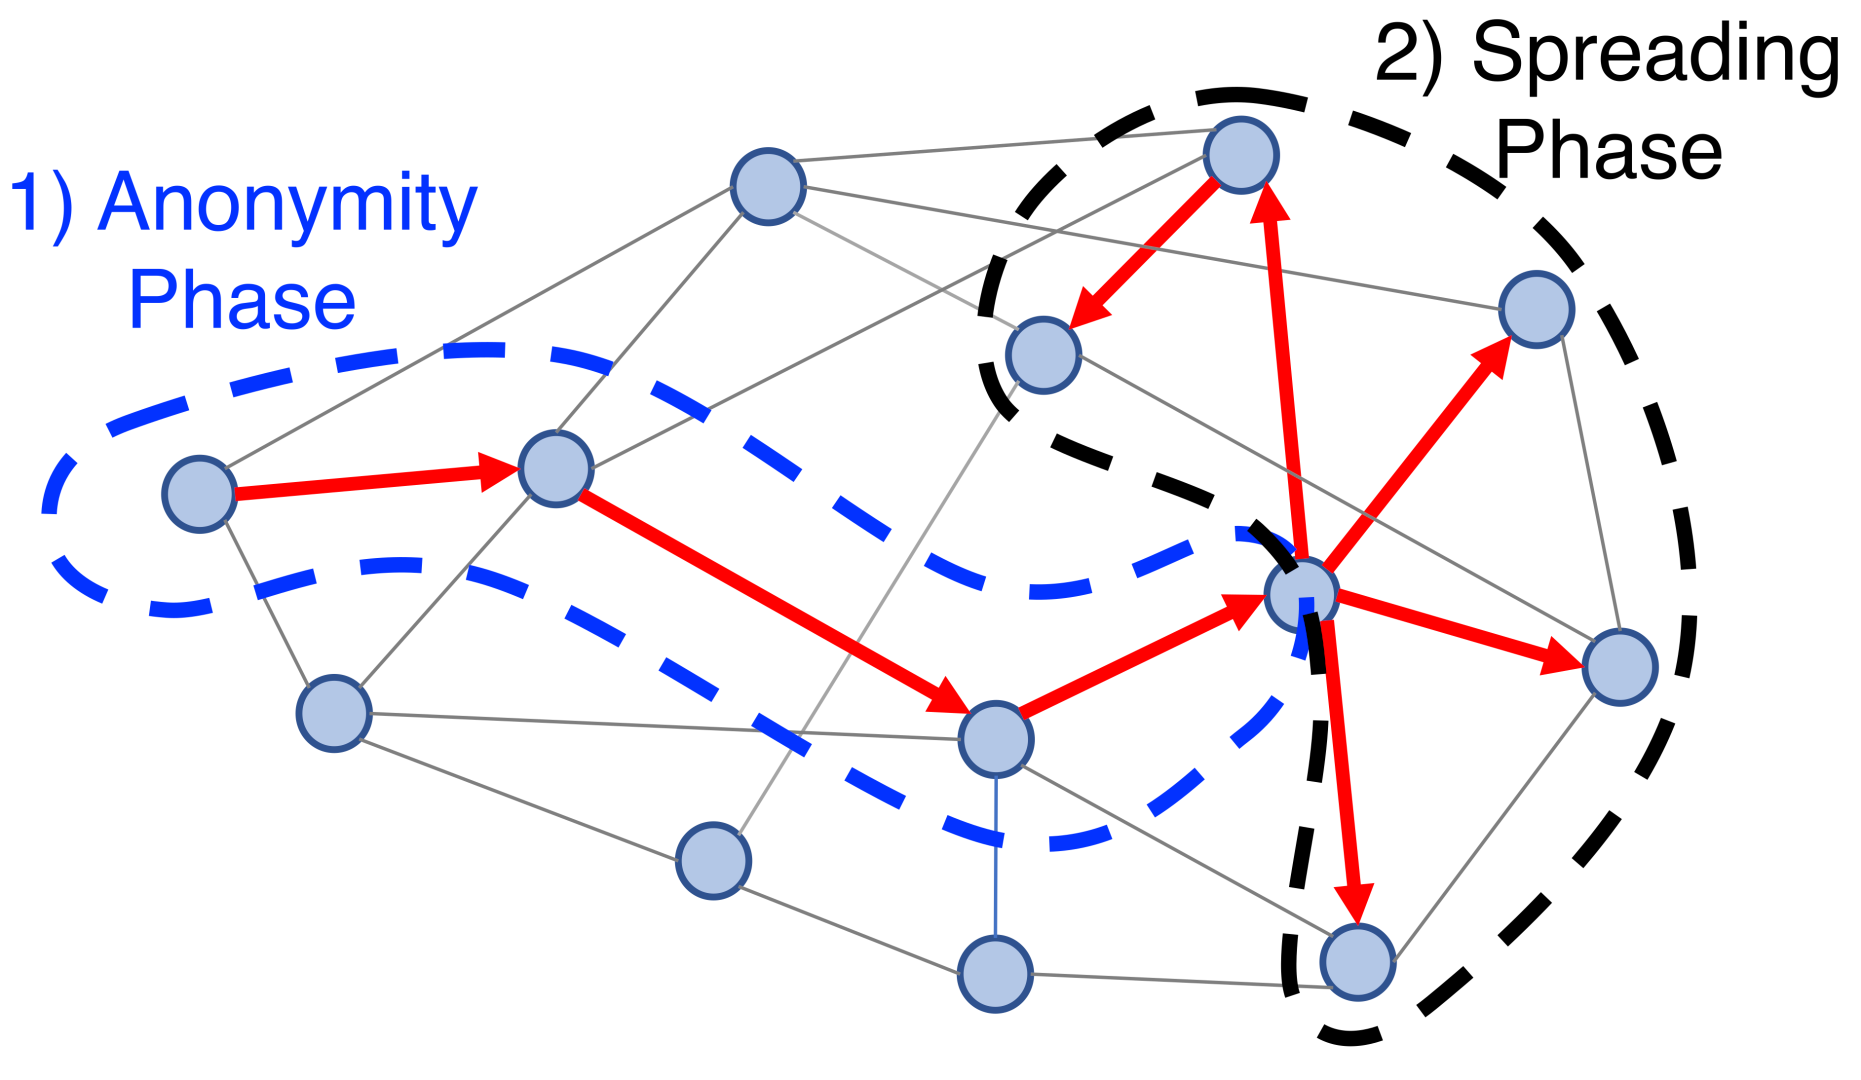
\includegraphics[height=160px]{dandelion}
    \caption{
        Phases of Dandelion Transaction Propagation\\
        Image source: ``Dandelion'' protocol white paper\cite{dandelion_original} 
    }
    \label{fig:dandelion}
\end{figure}

\noindent\textbf{``Stem'' Anonymity Phase}
In this phase, a 4-regular\footnote{a 4-regular graph is a graph in which every vertex is connected to exactly four other vertices.} anonymity graph of nodes are created (and re-generated every epoch)\cite{dandelion}. If the node is committing a new transaction of its own, it forwards the transaction along the same outbound edge in the anonymity graph\cite{localmonero-dandelion}.

Each time a node receives a stem-phase transaction from another node it relays transactions to two pseudorandomly chosen peers according to a map of incoming and outbound edges in the anonymity graph\cite{dandelion}.

\medskip
\noindent\textbf{``Fluff'' Spreading Phase}
In the spreading phase, the node propagates transactions over the network via the conventional diffusion method, transmitting the transaction to all of its connected nodes. This broadcasts the transaction to every outgoing connection with randomized communication times\cite{dandelion_original}.

\medskip
This two-stage method of propagation obfuscation makes an attacker unable to simply listen for the direction of a transaction. The stem phase nodes will have distributed the transaction randomly meaning the originating node of the fluff phase is not the source of the original transaction, and it is unknown how many hops along the stem the transaction underwent prior to mass propagation\cite{localmonero-dandelion}.


% ------------------------------------------ %
\subsection{Local vs Remote Nodes}
Because the Monero blockchain is quite large and can take a significant amount of time to sync (especially if using a mechanical hard drive) Monero wallets can connect to a ``Remote node'' rather than using a local node\cite{moneropedia}. Remote nodes, also known as public nodes, are not without potential drawbacks, however. A malicious remote node can easily see your IP address (negating the effectiveness of Dandelion+) and associate it with the transaction, hide blocks to make it appear as though your wallet is up-to-date, and provide a list of already spent decoy addresses reducing the effectiveness of ring signatures\cite{localmonero-remotenode}.

Despite the potential privacy compromises, using a remote node always remains secure as nodes are unable to manipulate transactions or access your private keys\cite{localmonero-remotenode}. Any concern of IP address transaction linking can be mitigated through the use of Tor, I2P, or a centralized VPN service such as ``Mullvad VPN.'' Remote nodes are sometimes the only option for wallets on mobile devices such as phones, Chromebooks, or laptops with insufficient free storage space. Using a remote node and conventional wallet is still preferable to using a ``light wallet'' such as ``MyMonero'' as these wallets handle all synchronization on an external server which requires access to your private view key, which gives complete access to inbound transaction history, in addition to all the potential risks of a remote node\cite{localmonero-remotenode}.

Monero wallets, like the internally developed desktop wallet ``Monero-Wallet-GUI,'' give the easy option of automatically configuring a local node or selection of a remote node. For Wownero there is very little need to use a remote node currently as, due to the lower transaction volume and more recent launch date, the blockchain database is much smaller..


\subsubsection{TOR}
``TOR,'' or ``The Onion Router,'' is a technology originally developed by the U.S. Navy which provides users with \emph{layers} of anonymity by routing traffic through many nodes and, theoretically, requiring an attacker to compromise all the nodes used to discern the original IP address of a user.
Monero can optionally be integrated with Tor and setup tutorials are provided in the Monero git repo documentation\cite{monero_repo}. The Monero and Wownero daemons provides a convenient command flag to connect to a Tor proxy running on localhost
\\\centerline{EX: \texttt{--tx-proxy tor,127.0.0.1:9050,10}}

\smallskip
Wownero's popular ``Wowlet''\cite{wowlet} wallet software uses Tor implicitly by default requiring no action on the part of the end user at all. 



\subsubsection{I2P}
``I2P,'' or the ``Invisible Internet Project,'' is another optional privacy protocol which can be used. There has been discussion and interest in future I2P integration with the Monero daemon, possibly through Kovri (discussed in section \ref{sec:kovri}), however this has been delayed\cite{kovri_repo}. I2P is intended to protect you from passive network monitoring, so that anyone observing network traffic cannot tell that Monero is being used at all. The Monero developers prefer I2P over TOR because of its more decentralized routing protocol and asymmetric connections which mitigate 'timing attacks'\cite{monerohow_privacy}. Currently, the Wownero endorsed I2P router is i2p-zero\cite{i2pzero_repo}. As with Tor a command line flag is available to connect to an I2P proxy running on localhost
\\\centerline{EX: \texttt{--tx-proxy i2p,127.0.0.1:90000}}

\subsubsection{Kovri} \label{sec:kovri}
Kovri is a privacy-focused network layer that based on the I2P specification developed by the Monero Research Lab\cite{kovri_repo}. Kovri is not (yet) part of Monero however it may be added in a future update after a thorough evaluation and security audit\cite{moneropedia}. Because of Wownero's historically less stringent testing requirements Kovri could be implemented into Wownero ahead of Monero.

Kovri aims to be an easy to use, maintain, and review I2P router with extended functionality such as a ``hidden mode'' which would make I2P usage harder to detect by an internet service provider\cite{kovri_repo}. That feature could help to make Monero and Wownero more available in totalitarian countries with a highly controlled internet. Kovri is a rewrite of I2P in C++, forked from the i2pd project, for higher performance and to remove dependence on a bulky Java runtime\cite{kovri_repo}.

Their seems to be some hostility between I2P and Kovri developers as shown in the Kovri FAQ section ``Why did you fork from i2pd?'' \cite{kovri_repo}
\begin{quote}
    \dots We wanted a positive community that encouraged collaboration for the betterment of the software; not negative, narcissist glory\dots [and] a lead developer who could lead; not someone who could ignore requests for responsible disclosure or tuck-tail-and-run when faced with collaborator conflict
\end{quote}
Hopefully this disagreement will not jeopardize future development of either of these privacy-enhancing projects, however, the Kovri project may have been abandoned already as the last commit was 3 years ago and public enthusiasm towards the project has declined. 




\pagebreak
\section{Conclusion}
In conclusion, Wownero is a privacy-focused cryptocurrency, based on Monero but with a fixed supply, modifications to the block time, confirmation requirement, mining algorithm, emission profile, ring size, and its own unique software ecosystem and branding. In keeping with Monero's privacy and anonymity focused philosophy, Wownero's has many privacy features including stealth addresses, ring signatures, transaction amount hiding, network obfuscation, and integrations with proxy services such as TOR and I2P.

Wownero has faced challenges with mass adoption due to its privacy features reducing public exchange listings. Despite this, Wownero's development community is continuingly working on improving its software ecosystem of wallets and various integrations to make it more accessible, user-friendly, and useful.

Overall, Wownero is a promising cryptocurrency for those who value privacy, anonymity, and decentralization in their shitcoin transactions. Its unique features and development roadmap make it an interesting coin to follow, especially for those who are already familiar with Monero.
% ========================================== %

% Print Bibiligraphy Pages
% ========================================== %
%\pagebreak
\printbibliography
% ========================================== %


% Wownerochan image in bottom right corner
% ========================================== %
\tikz[remember picture, overlay] \node[anchor=south east] at (current page.south east) {
    
\includegraphics[width=4cm]{wownerochan}
};
% ========================================== %

\end{document}

% Notes and Examples
% ========================================== %
\iffalse

% Fandy Header
% ========================================== %
\usepackage{fancyhdr}
\pagestyle{fancy}
\setlength{\headheight}{15pt}
\fancyhead[L]{003128756}
\fancyhead[C]{\authorname}
\fancyhead[R]{\docdate}
% ========================================== %

% Pad to end of page
\vspace*{\fill}

% Numbered List
% ========================================== %
\begin{enumerate}
    \item list item
\end{enumerate}
% ========================================== %

% Draw line across full page
\noindent\hrulefill

% Show an image centered with caption
% ========================================== %
\begin{figure}[ht!]
    \centering
    \includegraphics[width=300px]{figurefile}
    \caption{
        A very important diagram\\
        Image source \texttt{init.cx} credit \emph{``rootinit''}
    }
    \label{fig:labelhere}
\end{figure}
% ========================================== %

\begin{align*}
    y^2 &= x^3+486662*x^2+x\\
    y &= -sqrt(x) sqrt(x^2 + 486662 x + 1)
    \end{align*}

    
\fi
% END